\documentclass[a4paper, 11pt]{report}
\usepackage{blindtext}
\usepackage[T1]{fontenc}
\usepackage[utf8]{inputenc}
\usepackage{titlesec}
\usepackage{fancyhdr}
\usepackage{geometry}
\usepackage{fix-cm}
\usepackage[hidelinks]{hyperref}
\usepackage{graphicx}
\usepackage{multirow}
\usepackage[english]{babel}

\geometry{ margin=30mm }
\counterwithin{subsection}{section}
\renewcommand\thesection{\arabic{section}.}
\renewcommand\thesubsection{\thesection\arabic{subsection}.}
\usepackage{tocloft}
\renewcommand{\cftchapleader}{\cftdotfill{\cftdotsep}}
\renewcommand{\cftsecleader}{\cftdotfill{\cftdotsep}}
\setlength{\cftsecindent}{2.2em}
\setlength{\cftsubsecindent}{4.2em}
\setlength{\cftsecnumwidth}{2em}
\setlength{\cftsubsecnumwidth}{2.5em}


\begin{document}
\titleformat{\section}
{\normalfont\fontsize{15}{0}\bfseries}{\thesection}{1em}{}
\titlespacing{\section}{0cm}{0.5cm}{0.15cm}
\titleformat{\subsection}
{\normalfont\fontsize{13}{0}\bfseries}{\thesubsection}{0.5em}{}
\titlespacing{\section}{0cm}{0.5cm}{0.15cm}

%=======================================================================================

% #########################
% IMPORTANT - Add student names here!
\newcommand{\studA}{{Aurelia, Serafina}}
\newcommand{\studB}{{Qin, Ziyi}}
\newcommand{\studC}{{Ng, Danison}}
\newcommand{\studD}{{Constantine, Matthew}}
%
% IMPORTANT - Then give your SIDs
\newcommand{\sidA}{{530805674}}
\newcommand{\sidB}{{540715325}}
\newcommand{\sidC}{{530683474}}
\newcommand{\sidD}{{530814528}}
%
% IMPORTANT - And then update which major each student will focus on
\newcommand{\majA}{{Computer Test}}
\newcommand{\majB}{{Computational Data Science}}
\newcommand{\majC}{{SW Development}}


\newcommand{\majD}{{Cyber Security}}
% #########################



\pagenumbering{Alph}
\begin{titlepage}
\begin{flushright}

\includegraphics[width=4cm]{USyd}\\[1cm]
\end{flushright}

\begin{centering}
\textbf{\huge INFO1111: Computing 1A Professionalism}\\[0.75cm]
\textbf{\huge 2024 Semester 1}\\[2cm]
\textbf{\huge Skills: Team Project Report}\\[2cm]

\textbf{\large Submission number: 1}\\[0.5cm]
\textbf{\large Github link:} \href{https://github.sydney.edu.au/dang3604/INFO1111_2024}{https://github.sydney.edu.au/dang3604/INFO1111_2024}\\[0.75cm]
\textbf{\huge Team Members:}\\[0.75cm]

\begin{tabular}{|p{0.25\textwidth}|p{0.13\textwidth}|p{0.12\textwidth}|p{0.12\textwidth}|p{0.22\textwidth}|}
	\hline
	\multirow{2}{*}{Name} & \multirow{2}{*}{Student ID} & Target * & Target * & \multirow{2}{*}{Selected Major} \\
	 & & Foundation & Advanced & \\
	\hline
	\hline
	\raggedright{\studA} & \sidA & A & NA & \majA \\
	\hline
	\raggedright{\studB} & \sidB & A & NA & \majB \\
	\hline
	\raggedright{\studC} & \sidC & A & NA & \majC \\
	\hline
	\raggedright{\studD} & \sidD & A & NA & \majD \\
	\hline
\end{tabular}
\\[0.5cm]
\end{centering}

* Use the following codes:
\begin{itemize}
\setlength\itemsep{0em}
\item NA = Not attempting in this submission
\item A = Attempting (not previously attempting)
\item AW = Attempting (achieved weak in a previous submission) 
\item AG = Attempting (achieved good in a previous submission)
\item S = Already achieved strong in a previous submission
\end{itemize}

\thispagestyle{empty}
\end{titlepage}
\pagenumbering{arabic}


%=======================================================================================

\tableofcontents

%=======================================================================================

\newpage

\section{Task 1 (Foundation): Core Skills}

\subsection{Skills for \majA: \studA}


\section*{\textbf{Software Design}}
When applying computer science in the tech industry, we mainly focus on development of software applications. Therefore, we need software design as one of our main technical skills as a computer science graduate. Software design is the basis for all construction of larger systems that work together in tandem. By having software design skills, we can make sure a system is adaptive and works well with users without the need of high-level maintenance. This skill is the foundation for all software systems and has high impact on the overall quality of our program – making it the most critical skill to obtain to work in the computer science. industry\\

\section*{\textbf{Programming/Software Development (PROG)}}
Programming/software development comes right after software design. We create our system’s structure through software design and start on its implementation through this skill. It mainly comprises of coding, reviewing, documenting, and debugging based on the given specifications. Without programming/software development, we will never have an end product that can be given to clients. The development process also includes peer-review techniques to encourage contribution between experts in the industry. As this is one of final steps a product will go through before it launches, completing this process will increase the likelihood of product success.\\

\section*{\textbf{Problem Management (PBMG)}}
Problem management occurs very often in our lives – an easy example would be solving a disagreement in group works. However, in some cases, problem management might not be as intuitive since it requires a lot of critical thinking. When this skill is applied to the computer science industry, it is not as simple to identify potential bugs and errors in a software. This skill encompasses not only the technical coding side but also its relations to humans when we’re working with our future team at work. By practicing problem management, we can prevent future incidents from taking place. Additionally, problem management can be used in optimizing algorithms that decreases operating costs. While problem management is crucial, it is often done after software design is completed.
\subsection{Skills for \majB: \studB}

\section*{\textbf{Data science (DATS)}}
Data science DATS as one of the skills in skills framework for information age SFIA Is the most required skill for Computational data science. Computational data science focus on the ways for managing, organising, modelling and analyse of data, and eventually making solution for data-driven decision making. Data science involves the use of maths and statistics to predict output and producing output. Therefore, the skill In data science matches with the skill required such as data-driven decision making for Computational data science.

\section*{\textbf{Data management (DATM)}}
Data management DATM is also a skill listed in the SFIA. Data management is the skill of apply plans, rules and practices to produce the data output in most secured way. For example, collecting data from valid sources, making sure data are stored correctly, and apply certain rules when handling data. This skill is also an essential skill for the major of computational data science as understanding how to collect data is very useful at the initiative stage of doing a data science project, and storing data are also needed at the finishing stage of a data science project. 

\section*{\textbf{Data visualisation (VISL)}}
Data visualisation VISL, as a skill listed in the SFIA, are also a key skill to computational data science major. Data visualisation VISL involves the skill to display outputs using graphical ways, as well as presents pattern and trends of a list of data. Therefore, data visualisation makes the data communicates with the stakeholders in more efficient and understandable way. it also communicates in a more engaging ways to appeal the audience. Thus, making Data visualisation an essential skill in computational data science and an important skill for data scientists. 



\subsection{Skills for \majC: \studC}

\section*{\textbf{Coding Languages}}
Coding languages are an essential tool for software developers as they serve as a foundation for solving complex issues, building software, and facilitating collaboration between team members. Mastery of different coding languages allows developers to write efficient code for the organization, effectively reducing cost and time. Furthermore, knowing various languages enables developers to evaluate problems from different frameworks, fostering innovative solutions and enhancing the overall quality of software development projects. This versatility not only improves the efficiency of development processes but also opens up opportunities for developers to explore diverse avenues and stay adaptable.

\section*{\textbf{Change Control}}
Change control in software development ensures meticulous management of proposed changes to suit end-user needs, safeguarding the stability and integrity of products and services. By evaluating risks and implementing standardized procedures, teams minimize disruptions while maintaining performance, security, and compliance with regional regulations. Automation streamlines workflows, enabling continuous integration and timely updates. Effective change control can ensure the team of developers is working as a collective entity.

\section*{\textbf{Machine Learning}}
As machine learning becomes more prominent in developers' workflows, it is ever more important to ensure that machine learning techniques are integrated seamlessly into software engineering practices. Machine learning empowers software engineers to create intelligent systems capable of learning from data, making predictions, and adapting to changing environments. By leveraging ML algorithms, engineers can automate tasks, enhance user experiences, and unlock valuable insights from vast amounts of data. This integration not only enables the development of innovative solutions but also enhances efficiency, and scalability. Furthermore, the ability to utilize machine learning could be a competitive skill trait to have.




\subsection{Skills for \majD: \studD}


\section*{\textbf{Information Security (SCTY)}}

Information security is the protection of data from unauthorised access usually within the digital environment. This is the most important core tech skill as it the core foundation of every industry. Data must be protected at all costs to avoid data misuse and data lost. Data is the most important part of a company, as it holds the companies identity, and refers to many private, sacred and crucial information such as: passwords, bank accounts, data privacy, systems, industrial information , legislations and more. Without proper data protection, A company’s reputation, organisation and work will be all gone. To acquire this skill, a person must learn how to protect their data from potential leaks. This is a very complex skill as one has to be very meticulous in protecting data. It is divided into a red and blue team, where one has to protect and the other would try to find leaks. This team will help strengthen the security system for all information by constant updates and improvements. Hence, this core skill is a fundamental must when learning cybersecurity. This skill requires and holds the most responsibilities out of the other two chosen skills I chose.\\

\section*{\textbf{Incident Management (USUP)}}

Coming from security, incident management is the second most important core skills of a cybersecurity specialist. When data is breached, there must be countermeasures and responses by a team to mitigate in order to lessen the consequences. Information should also be spread to warn and inform others from potential threats. This is a really important skill, and serves as how to take responsibility if the information security fails. A team would need to make sure to lessen the damaging impact of a data breach or lost in order to allow a company to stay strong. Another part of importance is the capability to learn from past mistakes and enhance possible countermeasures for future problems. Incident management focuses on mitigating damages , counter measuring data breaches and rebuilding protection from incidents. They also conduct research from past incidents and provide improvements in cybersecurity while re-evaluating their own. Hence why this is a really important skill for cybersecurity.\\

\section*{\textbf{Risk Management (BURM)}}

Lastly, the third most important skill is risk management. After a strong system, and great mitigation skills, one must also keep updating and preparing for future threats. Risk management deals with compliance handling, management of future risks and consequences, and developing a safe path of improvement from other divisions.  This skill is important and pairs really well with the information security skill, as risk management handles all potential risks a company must comply to make sure everything runs safely. Risk Management can be seen from the preparation of company choices, measurements of strategies, analysing future potential risks and cost or time reduction methods. This is the third most important skill as with all three cybersecurity core skills, people are able to handle the current situation, the past situations and future situation.\\
>>>>>>> 8b6aa526221453d2470f334ff77b168dc586b870

% ========================================================

\newpage
\section{Task 2 (Advanced): Advanced Skills}

Task 2 contains two components (both required).\\[2mm]

\textbf{Component 1: Exploration of Tech Tools}

The first component focuses on exploration of relevant tech tools used within professional computing employment. All companies make use of a range of technologies and tools (often as part of a tech stack). These tools might be implementation languages; design tools; data analysis tools; collaboration technologies, etc. Each student should identify two tools that are widely used in industry, and which relate to the major you are focusing on for this project. You should then describe:

\begin{enumerate}
\item What are the two tools you have identified for your chosen major
\item The main functionality of those tools;
\item The ways in which those tools are used in the industry of your chosen major;
\item Any weaknesses or limitations of those tools.
\end{enumerate}

This task consists of two parts:

\begin{enumerate}
\item \textbf{Part A}: Generate a set of questions that you can put to ChatGPT in order to obtain answers to each of the above four questions. Using ChatGPT, then generate the answers for each of the two tools. You must include in the report below both the questions that you posed to ChatGPT, and the answers that it provided.  (100–250 words each).
\item \textbf{Part B}: For each of the four answers from Part A, assess the answer that ChatGPT provided and explain to us why you agree or disagree with the answer (100 words for each question above).
\end{enumerate}


As examples of the tools which might be selected (which you shouldn’t now use):
\begin{itemize}
\item Computer Science: Eclipse.
\item Software Development: GitHub. 
\item Cyber Security: Wireshark. 
\item Data Science: Hadoop.
\end{itemize}

Note also that no two students in the same tutorial should choose the same tools, so your tutor will maintain a list of those that have already been selected. You should therefore check this list with your tutor and then confirm your choice with your tutor prior to researching your proposed tools and spending time writing about them. (Target = $\sim$200-400 words per tool).\\[2mm]

\textbf{Component 2: Advanced LaTeX and Git Skills}

The second component of Task 2 focuses on more advanced technical skills in LaTeX and Git. The following is a list of advanced Git and LaTeX skills/features. Each student in your team that is attempting the Advanced task should select a different pair of items from each list (e.g. you might choose ''Resetting and Tags'' from the git list, and ''Cross-referencing and Custom commands'' from the LaTeX list). You then need to demonstrate actual use of each item (either through activity in Git, or through including items in this report). (Target = $\sim$100-200 words per student for each feature).

\begin{enumerate}
\item{Git}
	\begin{enumerate}
	\item Rebasing and Ignoring files 
	\item Forking and Special files 
	\item Resetting and Tags 
	\item Reverting and Automated merges 
	\item Hooks and Tags 
	\end{enumerate}
\item LaTeX 
	\begin{enumerate}
	\item Cross-referencing and Custom commands 
	\item Footnotes/margin notes and creating new environments 
	\item Floating figures and editing style sheets 
	\item Graphics and advanced mathematical equations 
	\item Macros and hyperlinks
	\end{enumerate}
\end{enumerate}
~\\[2mm]

\textbf{OVERALL REQUIREMENTS:}

To achieve an ''OK'' rating for this task you must individually accomplish the following:
\begin{itemize}
\item \textbf{Component 1 - Exploration of Tech Tools}
	\begin{itemize}
	\item Identified two tools that are widely used in industry, and which relate to the major chosen for this project.
		\begin{itemize}
		\item The two tools selected are not the same as the tools selected by other students in the tutorial. 
		\item The two tools selected are relevant to the major chosen.
		\end{itemize}
	\item Answer the following questions as instructed in 'Part A' \& 'Part B':
		\begin{itemize}
		\item What are the two tools you have identified for your chosen major
		\item 3 main functionality of each of the identified tools
		\item The ways in which those tools are used in the industry of your chosen major;
		\item 2 weaknesses or limitations of each of the tools
		\end{itemize}
	\item \textbf{Part A}: Generate a set of questions (minimum 5 questions) that can be put to ChatGPT in order to obtain answers to each of the above four questions. Using ChatGPT, then generate the answers for each of the two tools. You must include in the report below both the questions that you posed to ChatGPT, and the answers that it provided. (100 - 250 words for each question)
	\item \textbf{Part B}: For each of the four answers from Part A, assess the answer that ChatGPT provided and explain to us why they agree or disagree with the answer (100 words for each question above).
	\end{itemize}
\item \textbf{Component 2 - Advanced LaTex \& Git Skills}
	\begin{itemize}
	\item Each member of the team has selected one pair of items from each list below and demonstrate actual use of each item (i.e. a Git item and a LaTeX item).
	\item \textbf{Git}
		\begin{itemize}
		\item Rebasing and Ignoring files
		\item Forking and Special files
		\item Resetting and Tags
		\item Reverting and Automated merges
		\item Hooks and Tags
		\end{itemize}
	\item \textbf{LATEX}
		\begin{itemize}
		\item Cross-referencing and Custom commands
		\item Footnotes/margin notes and creating new environments
		\item Floating figures and editing style sheets
		\item Graphics and advanced mathematical equations
		\item Macros and hyperlinks
		\end{itemize}
	\item This means no two members of the team have not chosen the same item from either of the lists above.
	\item You have demonstrated the use of your selected items either through activity in Git, or through including items in this report.
	\item This means for Git items:
		\begin{itemize}
		\item You have added your tutor to your git repository and when they view it they are able to see your activity that demonstrates the use of your selected items (e.g. forks, hooks, tags, merges etc.).
		\item You have included screenshots and annotations (where necessary) in your report and provided an explanation of $\sim$100 words of your use of advanced Git features.
		\end{itemize}
	\item and for LaTeX items:
		\begin{itemize}
		\item You have included items you have chosen in your LaTeX report document submission and the tutor is able to clearly see it (e.g. the pdf document written in LaTeX has hyperlinks, macros, cross referencing etc. included in it).
		\item You have included screenshots and annotations (where necessary) in your report and provided an explanation of $\sim$100 words of your use of advanced LaTeX features.
		\end{itemize}
	\end{itemize}
\item Referencing
	\begin {itemize}
	\item You have provided in-text references (IEEE) to support your claims or where they gathered the information from.
	\item You have a reference list following the IEEE referencing guidelines.
		\begin{itemize}
		\item Some common things to look for to see whether your have correctly followed the referencing guide are:
		\item Sources are listed in alphabetical order
		\item The sources you have listed are only the sources that are present in-text.
		\item All sources seen in-text are included in the reference list.
		\item You followed the correct convention for references that don’t have author’s details or multiple sources have the same author and year of publication
		\item You have included the required information for the source type as outlined in the guide.
		\item Sources are not a list (i.e. dotpoints)
		\end{itemize}
	\end{itemize}
\end{itemize}

To achieve a ''STRONG'' rating you must accomplish all of the above in addition to the following:
\begin{itemize}
\item The answers provided to the 4 questions (component 1b) use ChatGPT and independent research and analysis is excellent, showing a deep understanding of industry.
\item You have used advanced Git features such as branching when demonstrating the items you selected (component 2a).
\end{itemize}



% ========================================================

\subsection{Tools and Skills for \majA: \studA}

\subsubsection{Part A: Exploration of tech tools}

Your text goes here

\subsubsection{Part B: Analysis}

Your text goes here

\subsubsection{Technical Skills (LaTeX and Git)}

Your text goes here


% ========================================================

\subsection{Tools and Skills for \majB: \studB}

\subsubsection{Part A: Exploration of tech tools}

Your text goes here

\subsubsection{Part B: Analysis}

Your text goes here

\subsubsection{Technical Skills (LaTeX and Git)}

Your text goes here

% ========================================================

\subsection{Tools and Skills for \majC: \studC}

\subsubsection{Part A: Exploration of tech tools}

Your text goes here

\subsubsection{Part B: Analysis}

Your text goes here

\subsubsection{Technical Skills (LaTeX and Git)}

Your text goes here


% ========================================================

\subsection{Tools and Skills for \majD: \studD}

\subsubsection{Part A: Exploration of tech tools}

Your text goes here

\subsubsection{Part B: Analysis}

Your text goes here

\subsubsection{Technical Skills (LaTeX and Git)}

Your text goes here


%=======================================================================================

\newpage
\section{Submission contribution overview}
Our contributions throughout the project.

\subsection{Submission 1 contribution overview}


During one of our tutorial sessions, we managed to figure out how to push and pull files from github. Since then, we did each of our parts accordingly during our own time. The following week, we met up outside our tutorial sessions to finalize the formatting of the document. We each committed and pushed our files to the github repository, and everyone else 
was succesfully able to pull it. Everyone was present during the meeting and contributed equally. We aimed to get the strong rating for this task, so we made sure to include the extra evidence required as well.\\
\begin{figure}[h]
    \centering
    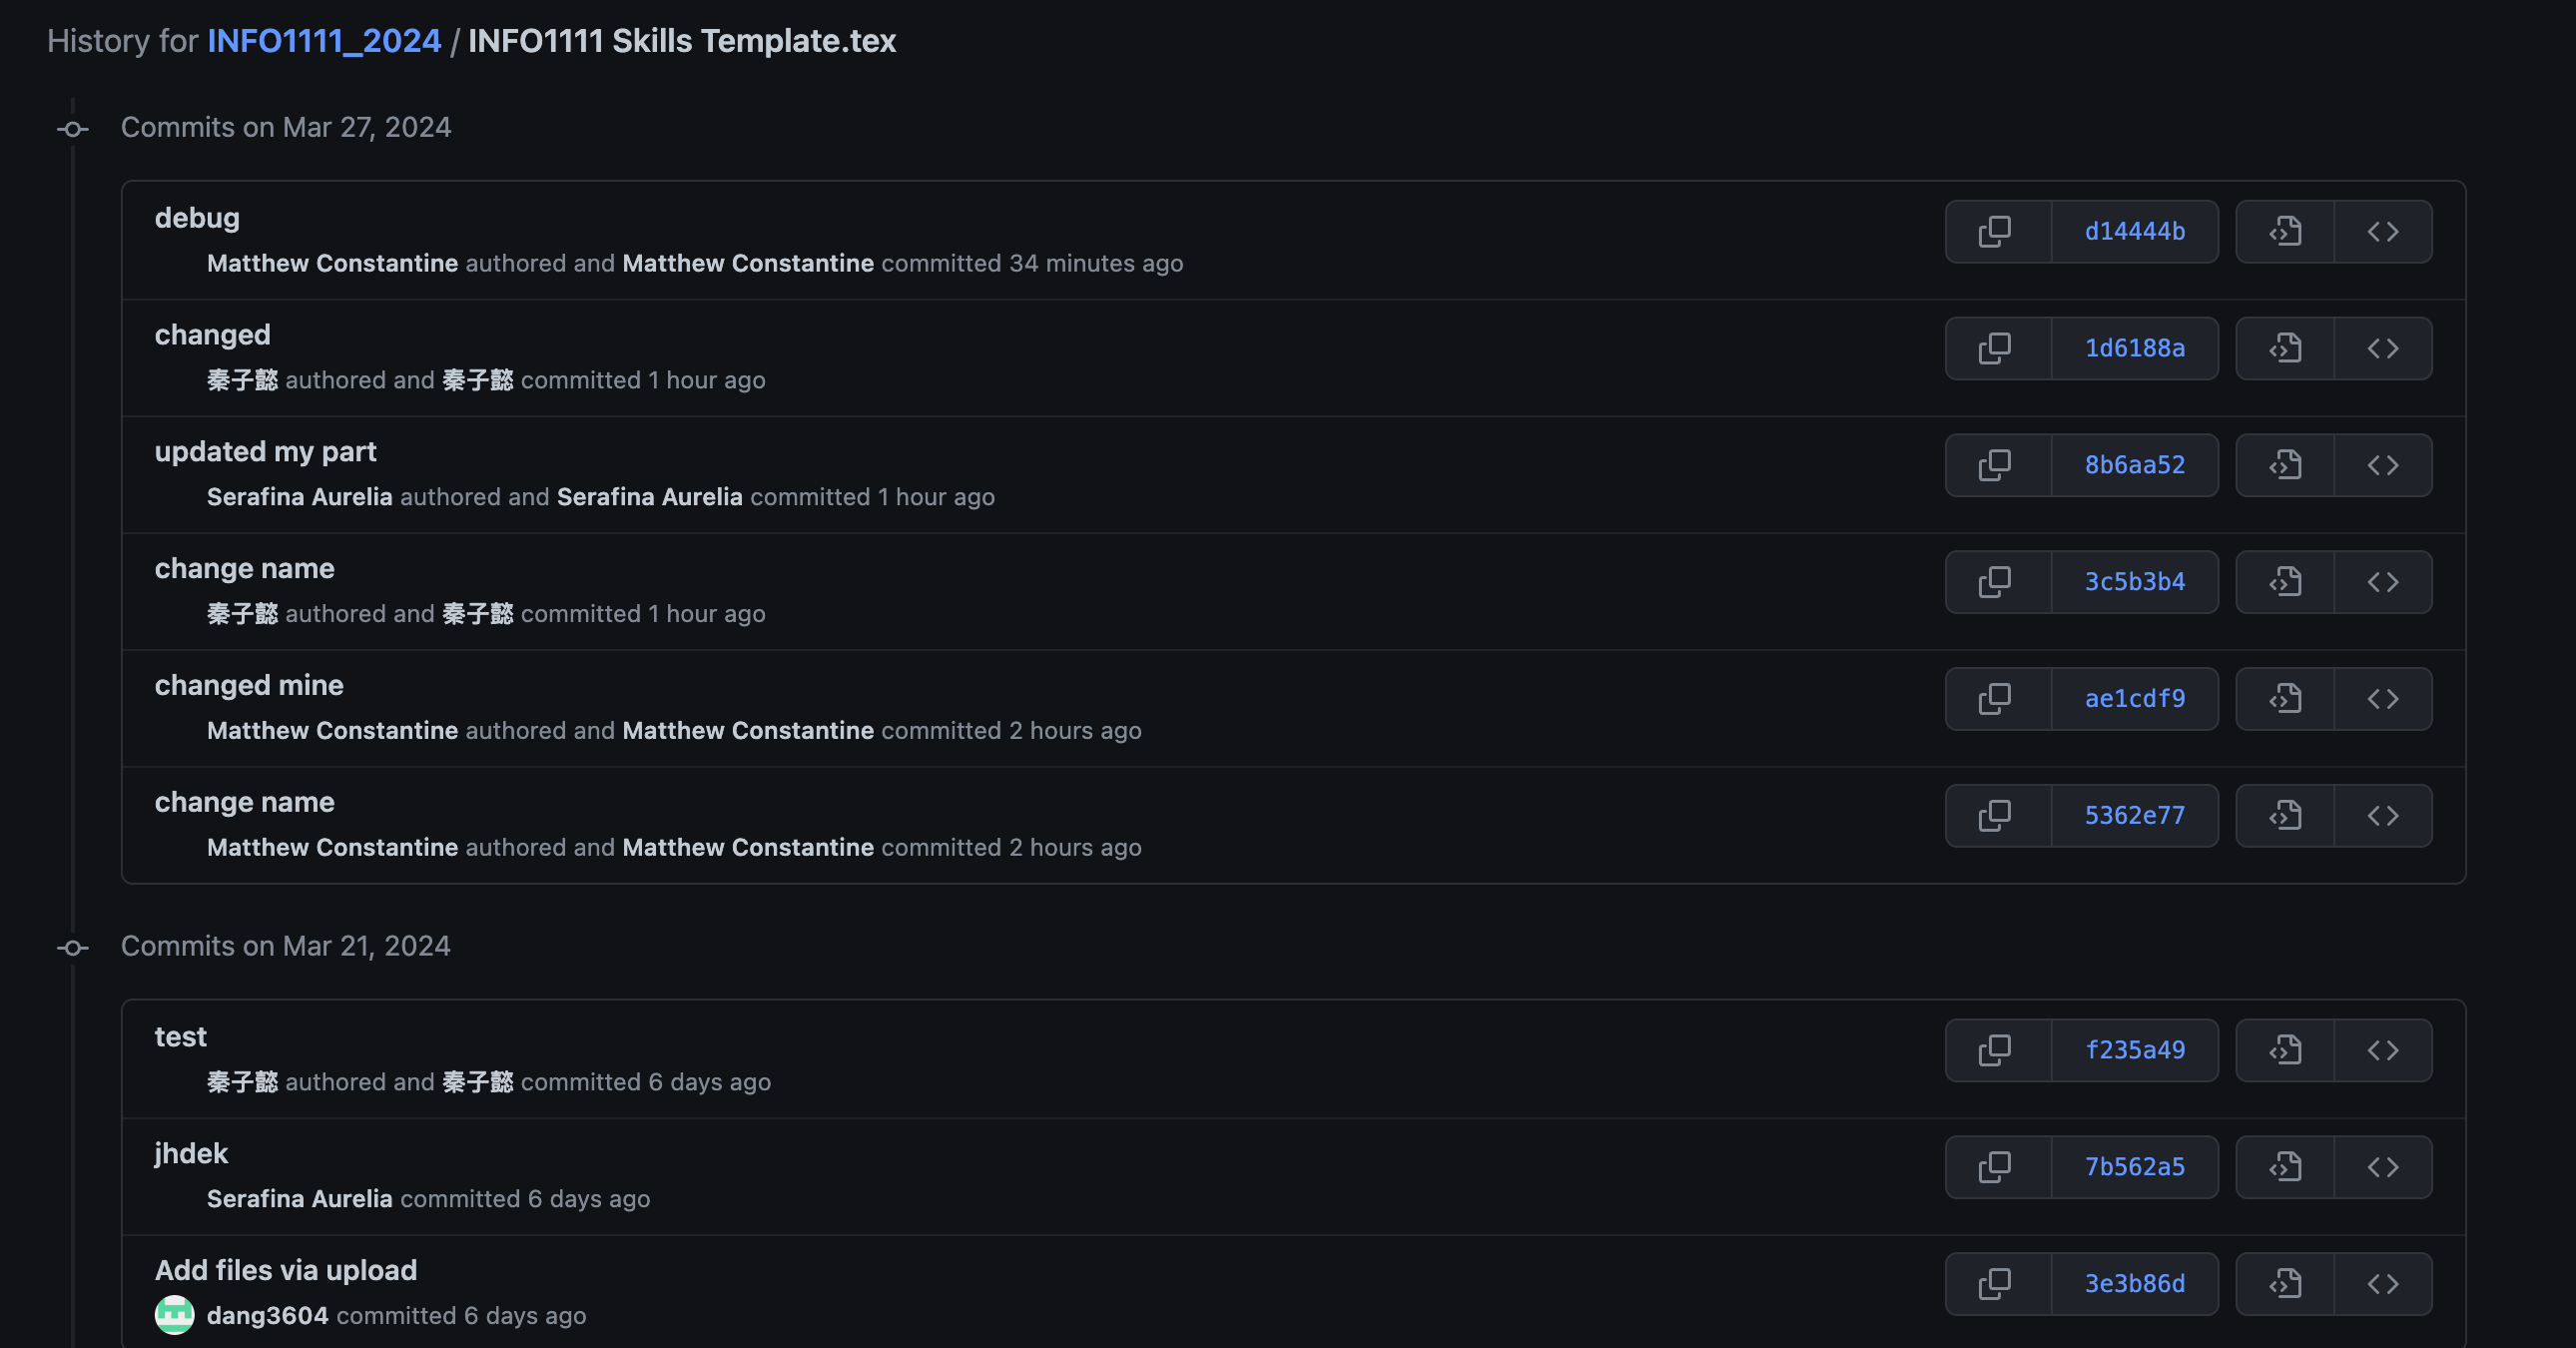
\includegraphics[width=0.5\linewidth]{commits.png}
    \caption{Commit History}
\end{figure}

\begin{figure}[h]
    \centering
    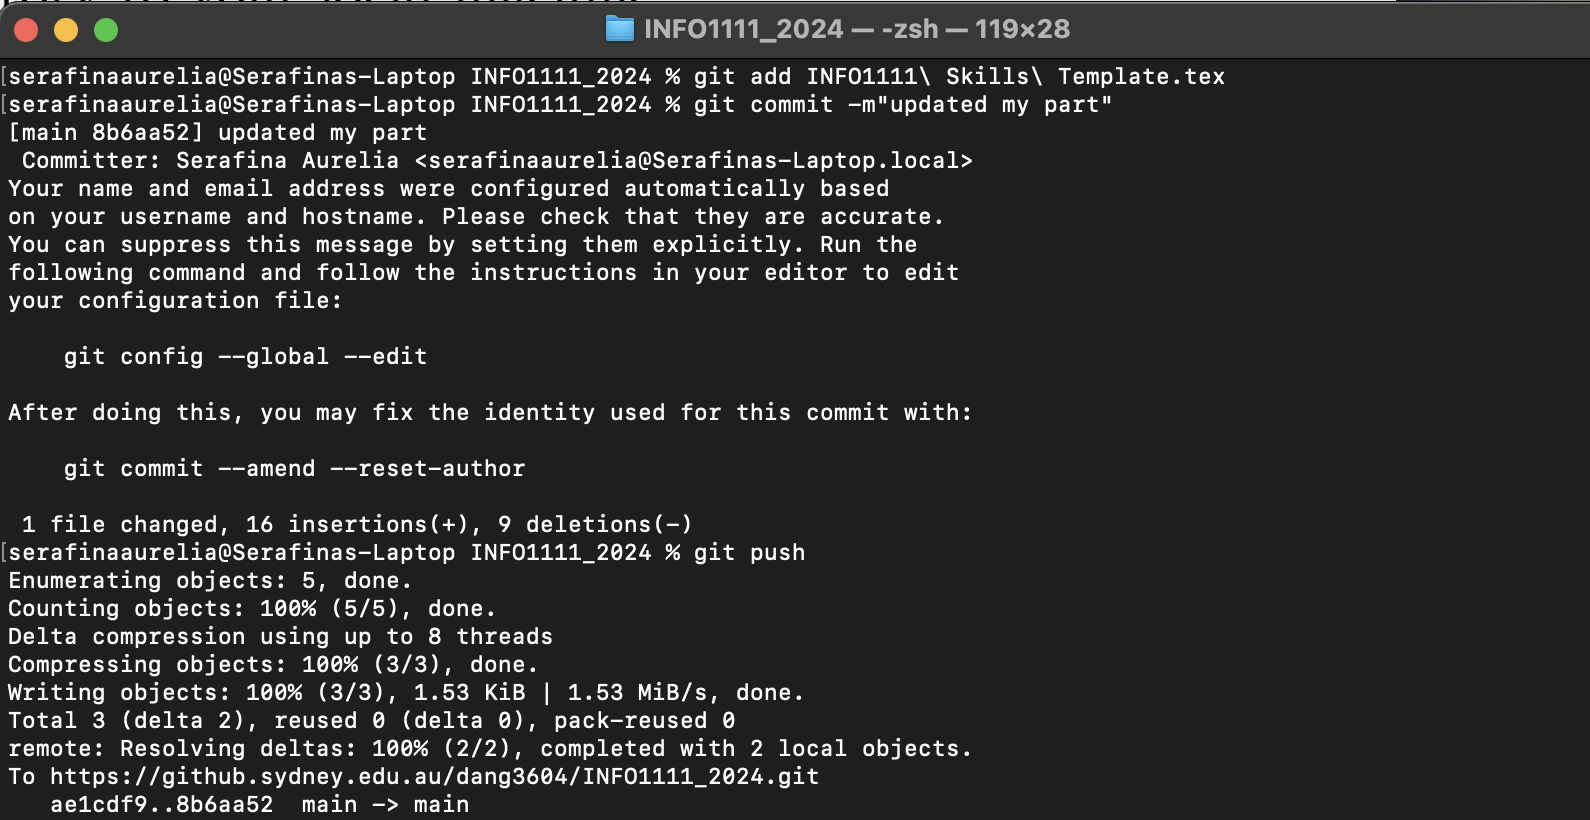
\includegraphics[width=0.5\linewidth]{push.png}
    \caption{Pushes}
\end{figure}

\begin{figure}
    \centering
    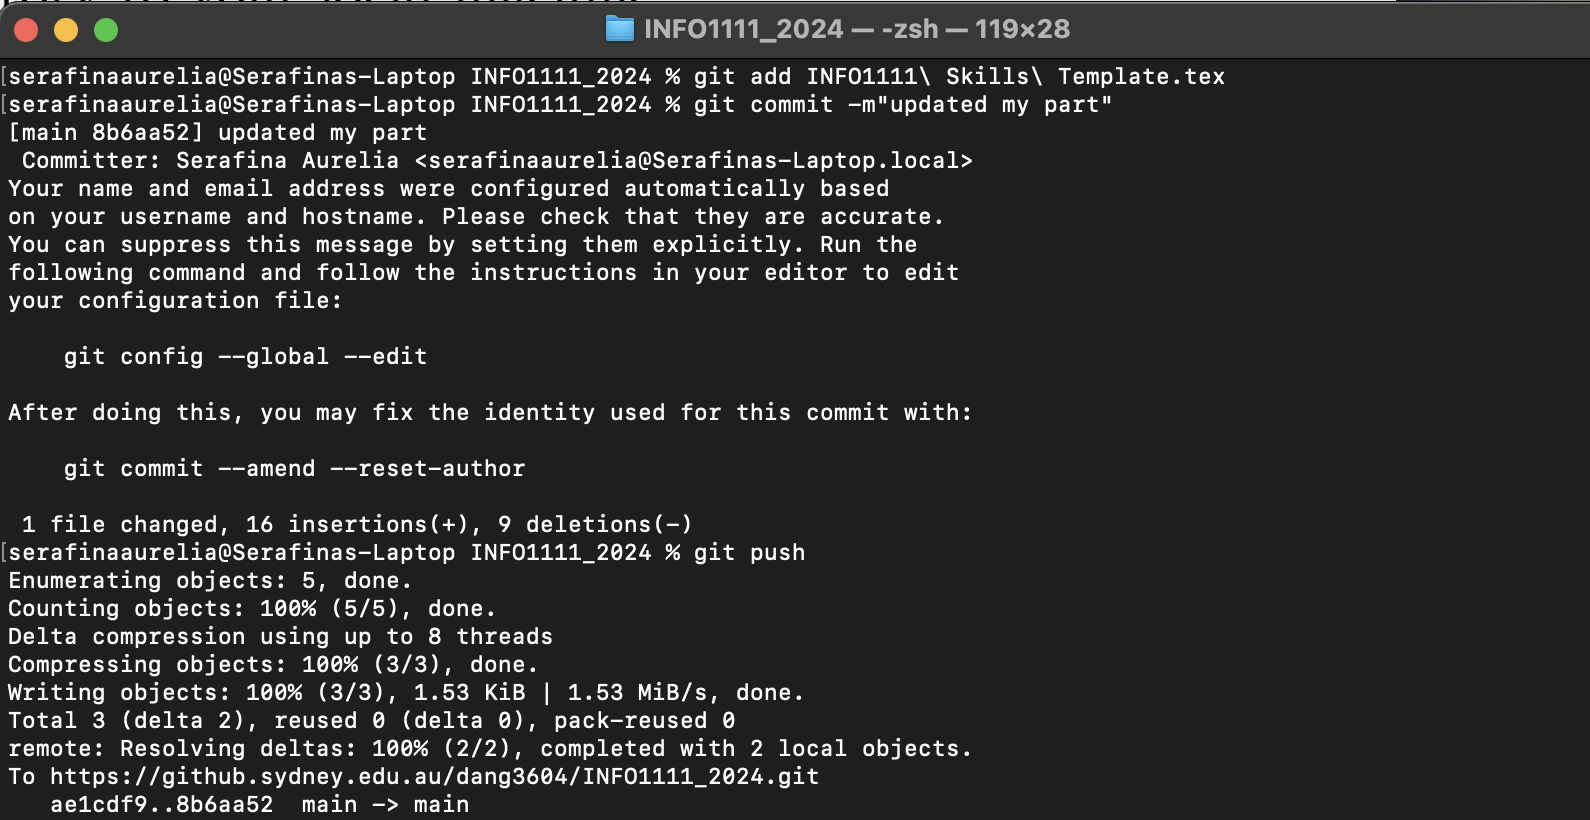
\includegraphics[width=0.5\linewidth]{pull.png}
    \caption{Pulling for collaboration}
\end{figure}


\subsection{Submission 2 contribution overview}

As above, for submission 2

\subsection{Submission 3 contribution overview}

As above, for submission 3


%=======================================================================================

\newpage

\bibliographystyle{ieeetran}
\bibliography{main}

\end{document}
\end{report}